\documentclass[a4paper,french,12pt]{report}
\usepackage[utf8]{inputenc} % Encodage du fichier
\usepackage[T1]{fontenc} % Encodage des fonts nécessaire pour le Latin
\usepackage[frenchb]{babel} % Pour changer la langue des mots générés et choisir la bonne mise en page
\usepackage{lmodern} % Le latin modèrne
\usepackage[top=2cm, bottom=2cm, left=3cm, right=2cm]{geometry} % Définir les marges de la page
\usepackage{amsmath} % Pour des fonctions mathématiques
\usepackage{amssymb} % Pour les symbols mathématiques
\usepackage[hidelinks]{hyperref} % Pour les liens
\usepackage{fancyhdr} % Pour le style de la page
\usepackage[font=it]{caption} % Rendre le titre des tableaux italique
\usepackage{microtype}
\usepackage{graphicx} % Pour les images
\usepackage{subcaption} % Pour mettre plusieurs images sur la même ligne
\usepackage[section]{placeins} % Pour empêcher le déplacement des tableaux et des figures.
\graphicspath{ {pictures/} } % Spécifier le répertoire contenant les images  
\DisableLigatures[f]{encoding=*}
\renewcommand \thechapter{\Roman{chapter}} % Utiliser la numéros romans pour les chapitre
\AtBeginDocument{% Changer "Table"
  \renewcommand\tablename{\itshape Tableau}
  \renewcommand{\figurename}{\itshape Figure}
}
% Pour la 1ère page
\title{Le mémoire}
\author{Hamza Abbad \and Ahmed Zebouchi}
\date{}
% Style de l'entête et le pied de la page 
\setlength{\headheight}{16pt}
\pagestyle{fancyplain}
\lhead{} % Enlever la section
\rhead{\fancyplain{}{\nouppercase{\leftmark}}} % Titre du chapitre en miniscule
\cfoot{} % Déplacer le numéro de la page
\rfoot{\fancyplain{\thepage}{\thepage}} % à droite de la page
% Afficher les chapitres et les sections seulement
\setcounter{tocdepth}{1}
% Espace entre les lignes
\linespread{1.3}
\begin{document}
\maketitle
\tableofcontents
\parskip=0.6em
\chapter{Théorie de Dempster and Shafer}

\phantomsection
\addcontentsline{toc}{section}{Introduction}
\section*{Introduction}

La théorie de Dempster-Shafer, également connue comme la théorie de l'évidence,
ou théorie des fonctions de croyance, est une théorie mathématique du raisonnement
sur l’évidence et la plausibilité. Elle a été développée par Glenn Shafer (1976)
en se basant sur des travaux antérieurs de Arthur Dempster (1968). Elle a attiré
l’attention des chercheurs de l'intelligence artificielle au début des années 80.

Dans un espace discret fini, la théorie de Dempster-Shafer représente la généralisation
de la théorie des probabilités dans laquelle les probabilités sont assignées à des ensembles,
contrairement aux singletons mutuellement exclusifs.

\section{Concepts de base}

\subsection{Quelques notations}

Nous allons présenter ici les conventions de notation utilisées dans la suite de ce mémoire.

Soit $\Omega$ un univers constitué d'un ensemble fini qui contient toutes les propositions
auxquelles on s'intéresse, appelé également cadre de discernement. On note $\varnothing$
l’ensemble qui ne contient aucun élément de $\Omega$. $\mathcal{P}(\Omega)$ représente
l’ensemble contenant toutes les parties (les sous-ensembles) de $\Omega$. On note aussi
les opérations binaires sur les ensembles $\subset$, $\cup$ et $\cap$, qui sont l’inclusion,
l’union et l’intersection, respectivement. On appelle hypothèse un élément de $\mathcal{P}(\Omega)$.

La théorie de Dempster-Shafer est caractérisée par trois fonctions principales :
\textbf{l’assignement de probabilité de base} (\emph{basic probability assignement bpa}),
\textbf{la croyance} (\emph{belief}) et \textbf{la plausibilité} (\emph{plausibility}).

\subsection{L’assignement de probabilité de base}

Appelé aussi la fonction de masse, noté $m$, c'est une fonction qui affecte le degré d’évidence
disponible à un élément $A$, et seulement à $A$, de $\mathcal{P}(\Omega)$ dans l’intervalle
$[0,1]$, tel que les $m(A)$ s’additionnent à $1$.

$m(\varnothing)$ --qui représente l’absence
de solution-- est toujours égale à $0$ car $\Omega$ doit être exhaustive, et la somme de $m(A)$
vaut $1$. Chaque élément A tel que $m(A) > 0$ est appelé élément focal.

Généralement, le bpa n’est pas un équivalent de la fonction de probabilités classique. En effet,
la valeur exacte de la probabilité (dans le sens classique) appartient à un intervalle borné par
deux valeurs qui sont \emph{la croyance} et \emph{la plausibilité}.

Formellement, on peut représenter cela par :
\begin{equation}
m : \mathcal{P}(\Omega) \mapsto [0,1]
\end{equation}
\begin{equation}
m(\varnothing) = 0
\end{equation}
\begin{equation} \label{somme_masses}
\sum_{A \in \mathcal{P}(\Omega)} m(A) = 1
\end{equation}

\subsubsection{Exemple}
Dans une enquête sur un incident de vol, trois personnes \textit{P1}, \textit{P2}, \textit{P3}
sont accusées. L’enquêteur pense à 30\% que P1 est le voleur, à 50\% que l’un des deux autres
personnes P2 ou P3, est le voleur, et à 10\% que P1 ou P3 le soit.\\
Le cadre de discernement s'écrit ainsi : $$\Omega = \{P1, P2, P3\}.$$
L'ensemble de parties de $\Omega$ est : $$\mathcal{P}(\Omega) = \{\varnothing, \{P1\}, \{P2\},
\{P3\}, \{P1, P2\}, \{P1, P3\}, \{P2, P3\}, \Omega\}$$
La distribution des masses s'exprime ainsi : $$m(\{P1\}) = 0.3, m(\{P2, P3\})  = 0.5,
m(\{P1, P3\}) = 0.1$$ et $$m(\Omega) = 1 - (0.3+0.5+0.1) = 0.1$$ à partir de l’équation \ref{somme_masses}.\\
Les masses des hypothèses restantes sont toutes égalles à $0$.

\subsection{La croyance}

La croyance est la quantité de confiance qui supporte une hypothèse $A$ de
$\mathcal{P}(\Omega)$, toutes parties comprises.\\
On la note $Cr(A$) ou plus souvent $Bel(A)$. Il est clair que $Bel(\varnothing)$
est nulle, et $Bel(\Omega)$ est toujours 1. Il faut noter que la croyance est une
mesure non additive, c’est-à-dire que $Bel(A) + Bel(\Omega - A) \neq 1$.

Formellement :
\begin{equation}
Bel(\varnothing)=0
\end{equation}
\begin{equation}
Bel(\Omega)=1
\end{equation}
\begin{equation}
Bel(A) = \sum_{B \slash B \subseteq A} m(B)
\end{equation}
\begin{equation}
\forall p,q \in \mathcal{P}(\Omega) \medskip Bel(p \cup q) \geq Bel(p) + Bel(q) - Bel(p \cap q).
\end{equation}
On peut aussi obtenir le bpa avec la fonction inverse suivante :
\begin{equation}
m(A) = \sum_{B \slash B \subseteq A} (-1)^{|A-B|} Bel(B),
\end{equation}
où $|A-B|$ est la différence des cardinalités entre les deux ensembles.

\subsubsection{Exemple}
En continuité de l'exemple précédent, on calcule la croyance de chaque hypothèse :

\begin{table}[h!]
\centering
\begin{tabular}{|l|l|}
\hline
Hypothèse $A$ & Croyance $Bel(A)$\\
\hline
$\varnothing$ & $0$ \\
\hline
$\{P1\}$ & $0.3$ \\
\hline
$\{P2\}$ & $0$ \\
\hline
$\{P3\}$ & $0$ \\
\hline
$\{P1, P2\}$ & $0.3 + 0 + 0 = 0.3$ \\
\hline
$\{P1, P3\}$ & $0.3 + 0 + 0.1 = 0.4$ \\
\hline
$\{P2, P3\}$ & $0 + 0 + 0.1 = 0.1$ \\
\hline
$\Omega$ & $1$ \\
\hline
\end{tabular}
\caption{Les croyances calculées à partir de la distribution de masses}
\end{table}

\subsection{La plausibilité}

La plausibilité représente la croyance qu’il est possible
d’affecté à une hypothèse $A$ de $\mathcal{P}(\Omega)$; autrement dit,
c’est la croyance affectée à A et aux hypothèses dont l'intersection
avec $A$ n’est pas vide. On la note $Pl(A)$. La valeur de la plausibilité est
toujours supérieure ou égale à celle de la croyance. Identiquement à la
croyance, $Pl(\varnothing)$ est nulle, et $Pl(\Omega)$ vaut $1$.

Formellement :
\begin{equation}
Pl(\varnothing) = 0
\end{equation}
\begin{equation}
Pl(\Omega) = 1
\end{equation}
\begin{equation}
Pl(A) = \sum_{B \slash B \cap A \neq \varnothing} m(B)
\end{equation}
La plausibilité peut aussi être dérivée à partir de la croyance:
\begin{equation}
Pl(A) = 1 - Bel(\bar{A}),
\end{equation}
où $A$ est le complément de $A$ dans $\Omega$.

La probabilité classique d’un événement $A$, $P(A)$ est représentée par
l’intervalle qui a comme bornes inférieure et supérieure $Bel(A)$ et $Pl(A)$,
respectivement, c’est-à-dire $$Pl(A) \leq P(A) \leq Bel(A).$$
Si $$Bel(A) = Pl(A),$$ alors la probabilité de $A$ est unique et $$P(A) = Bel(A) = Pl(A)$$

\subsubsection{Exemple}
On calcule les plausibilités pour le même exemple.

\begin{table}[h!]
\centering
\begin{tabular}{|l|l|}
\hline
Hypothèse $A$ & Plausibilité $Pl(A)$\\
\hline
$\varnothing$ & $0$ \\
\hline
$\{P1\}$ & $0.3 + 0.1 + 0.1 = 0.5$ \\
\hline
$\{P2\}$ & $0.5 + 0.1 = 0.6$ \\
\hline
$\{P3\}$ & $0.5 + 0.1 + 0.1 = 0.6$ \\
\hline
$\{P1, P2\}$ & $0.3 + 0.5 + 0.1 + 0.1 = 1$ \\
\hline
$\{P1, P3\}$ & $0.3 + 0.5 + 0.1 + 0.1 = 1$ \\
\hline
$\{P2, P3\}$ & $0.5 + 0.1 + 0.1 = 0.7$ \\
\hline
$\Omega$ & $1$ \\
\hline
\end{tabular}
\caption{Les plausibilités calculées à partir de la distribution de masses}
\end{table}
\section{Règles de combinaison}

Souvent, on obtient l’information à partir de sources distinctes et indépendantes,
et généralement ces sources ne sont pas parfaites, c’est pourquoi on a besoin de
fusionner les évidences fournies par ces sources en utilisant des règles de
combinaison. Il existe trois types de combinaison : \emph{conjonctive},
\emph{disjonctive}, et \emph{mixte}.

\subsection{Combinaison conjonctive}

Dempster a introduit une règle connue sous le nom de règle de combinaison
de Dempster (\emph{Dempster's Combination Rule}) pour fusionner deux pièces
d’évidence qui peuvent être représentées par deux fonctions de croyance.Cette
règle respecte les quatre propriétés algébriques suivantes : l’associativité,
la commutativité, l’idempotence et la continuité.

Soient deux fonctions de masse $m_1(A)$ et $m_2(A)$ associées à deux fonctions
de croyance $Bel_1(A)$ et $Bel_2(A)$ respectivement. $(Bel_1 \oplus Bel_2)(A)$
est définie à travers la masse $m_{1 \oplus 2}(A)$ :
\begin{equation}
m_{1 \oplus 2}(A) = \sum_{B \cap C = A} m_1(B) m_2(C).
\end{equation}

Néanmoins, cette règle a été critiquée par de nombreux chercheurs, parce qu’elle
n’est pas normalisée. En d’autre termes, elle permet d’affecter des masses à
des ensembles vides. Ce problème est dû au fait que l’intersection de deux
éléments focaux peut générer $\varnothing$, ce qui dénote un conflit entre les croyances.

Pour corriger ce problème, Shafer a proposé d’ignorer carrément les conflits
et d'étendre la distribution des masses. Le facteur de conflit est une valeur
$K < 1$ et définie par :
\begin{equation}
K = \sum_{B \cap C = \varnothing} m_1(B) m_2(C).
\end{equation}

Afin de normaliser la distribution de masse, la règle de Dempster doit être
multipliée par la quantité $(1 - K)^{-1}$. Donc la règle de Dempster-Shafer
est représentée par les équations suivantes :
\begin{equation}
m(\varnothing) = 0
\end{equation}
\begin{equation}
m(A) = \frac{1}{1-K} \sum_{B \cap C = A \neq \varnothing} m_1(B) m_2(C)
\end{equation}

Cependant, la règle de Shafer n’est pas toujours satisfaisante à cause de la
normalisation qui considère que le conflit vient de l’imperfection des sources.

D’autres chercheurs ont proposé des règles différents, comme Smets qui a introduit
une forme non normalisée pour prendre en compte les univers ouverts. Il suppose
que le conflit vient du fait que l’ensemble $\Omega$ n’est pas exhaustif. Pour
cette raison, la règle de Smets affecte une masse $K$ à $\varnothing$ qui représente
une hypothèse manquante. Elle est définie par ces équations :
\begin{equation}
K = m(\varnothing) = \sum_{B \cap C = \varnothing} m_1(B) m_2(C)
\end{equation}
\begin{equation}
m(A) = \sum_{B \cap C = A \neq \varnothing} m_1(B) m_2(C)
\end{equation}

Par contre, Yager propose un modèle d’un univers fermé ($\Omega$ est exhaustif).
La mesure de conflit est ajoutée à la mesure du cadre de discernement $\Omega$.
Donc le conflit sera transformé en ignorance. On obtient ces équations :
\begin{equation}
m(\varnothing) = \sum_{B \cap C = \varnothing} m_1(B) m_2(C)
\end{equation}
\begin{equation}
m(\Omega) = \left(1 - \sum_{A \in \mathcal{P}(\Omega)}
\sum_{B \cap C = A \neq \varnothing} m_1(B) m_2(C)\right) +
\sum_{B \cap C = \varnothing} m_1(B) m_2(C)
\end{equation}

\subsection{Combinaison disjonctive}

Dans la combinaison disjonctive on considère l’utilisation de l’union à la place
de l’intersection. Les éléments focaux sont obtenus à partir de la table d’union.
La fonction de masse de la règle de combinaison disjonctive est formalisée par l'équation :
\begin{equation}
m(A) = \sum_{B \cup C = A \neq \varnothing} m_1(B) m_2(C).
\end{equation}

Comme l’union de deux éléments focaux ne peut être jamais vide, on est sûr
que $m(\varnothing)=0$. Cela veut dire qu’il est impossible d’obtenir un conflit
lors de la combinaison. En contrepartie, l'union peut causer une perte de spécificité
vu que les masses sont élargies. Cette approche apparaît plus intéressante en
l’absence des informations nécessaires sur la fiabilité des sources.

\subsection{Combinaison mixte}

Dubois et Prade ont proposé une combinaison mixte comme un compromis entre la
combinaison conjonctive et la combinaison disjonctive et comme un essai de conserver
les avantages des deux. De même que la combinaison de Yager, le modèle de Dubois
et Prade suppose que le conflit est dû à la non fiabilité des sources. La règle de
Dubois et Prade est définie comme suit :
\begin{equation}
m(A) = \sum_{B \cap C = A \neq \varnothing} m_1(B) m_2(C) +
\sum_{\substack{B \cup C = A \neq \varnothing \\ B \cap C = \varnothing}} m_1(B) m_2(C)
\end{equation}

\section{Décision}

Prendre une décision veut dire choisir une hypothèse élémentaire parmi les autres
par la maximisation d'un critère. La sélection est établie en observant
la croyance et la plausibilité de chaque hypothèse résultante. Il existe trois règles
de décision : le \emph{maximum de croyance}, le \emph{maximum de plausibilité} et le
\emph{maximum de probabilité pignistique}

\subsection{Maximum de croyance}

Dans cette règle on s'intéresse à trouver l'hypothèse élémentaire $\omega_i$ qui
a la croyance maximale. C'est-à-dire que $\omega_i$ est choisie si elle satisfait cette
équation :
\begin{equation}
Bel(\omega_i) = \max_{1 \leq j \leq n} Bel(\omega_j)
\end{equation}
Cette méthode est connue par son caractère très pessimiste.

\subsection{Maximum de plausibilité}

En opposition à la règle précédente, l'élément $d_i$ est sélectionné par le maximum
de plausibilité. En d'autres termes, on choisit le $d_i$ qui résoud cette équation :
\begin{equation}
Pl(\omega_i) = \max_{1 \leq j \leq n} Pl(\omega_j).
\end{equation}
Ainsi, cette méthode a un caractère très optimiste.

\subsection{Maximum de probabilité pignistique}

Cette règle est proposée par Smets et Kennes. Elle consiste à transformer la fonction
de masse $m(A)$ en une fonction de probabilité $BetP(\omega)$. Cette transformation
est appelée \emph{transformation pignistique} et définie par cette équation :
\begin{equation}
BetP(\omega) = \sum_{\substack{A \subseteq \Omega \\
\omega \in A}} \frac{1}{|A|}  \frac{m(A)}{1-m(\varnothing)}.
\end{equation}

Dans cette transformation, la masse de croyance $m(A)$ est distribuée uniformément
sur l’ensemble des éléments de $A$. Le critère est de prendre l'élément qui a le
maximum de probabilité pignistique. On peut voir cette méthode comme un compromis
entre les deux précédentes.

\phantomsection
\addcontentsline{toc}{section}{Conclusion}
\section*{Conclusion}

Après cette présentation de la théorie des fonctions de
croyances, des règles de combinaisons qui peuvent si appliquer,
et des règles de décisions compatibles, nous allons maintenant pouvoir introduire
des notions sur les théories de l'incertain.
\chapter{Réalisation du \appname et de la \platformename}
\phantomsection
\addcontentsline{toc}{section}{Introduction}
\section*{Introduction}

Dans ce chapitre, nous introduisons l'implémentation de notre projet. D'abord, nous
citons les différents langages de programmation et les bibliothèques que nous avons manipulé.
Ensuite, nous présentons le \appname en détaillant ses fonctionnalités. Enfin, nous exposerons
la description de la \platformename qui regroupe plusieurs programmes reliés aux théories de
l'incertain. Nous expliquerons aussi comment cette plateforme interagit avec ces programmes.

\section{Les langages de programmation et les bibliothèques utilisées}

Nous avons programmé l'interface du \appname en \textbf{Python 3}
en utilisant la bibliothèque \textbf{PyQt4}. Nous avons également réalisé la \platformename
avec \textbf{Java Swing}. De plus, plusieurs scriptes utilisés par cette
plateforme sont écrits en \textbf{MATLAB}. D'autres outils sont programmés en langage
\textbf{C} et compilés sous une forme exécutable. Il y a aussi quelques programmes
qui nécessitent la présence de l'environement \textbf{Cygwin}.

\section{Le \appname}

Ce logiciel est constitué de deux parties, le noyau et l'interface graphique.
Il peut fonctionner sur tous les systèmes d'exploitation majeurs comme \textbf{Windows},
\textbf{\mbox{Mac OS X}}, \textbf{\mbox{GNU/Linux}} et \textbf{BSD}.

Le noyau est responsable d'effectuer les calculs après la lecture d'un fichier XML
contenant les données nécessaires pour l'application de la théorie de Dempster-Shafer.
Les résultats seront écrits dans un autre fichier XML. L'utilisateur n'a pas besoin
de comprendre la structure de ces fichiers, il lui suffit d'utiliser l'interface
graphique.

Cette interface est composée d'une barre de menu et de trois parties: les états
du monde, les hypothèses, et les agents. La barre contient les fonctionnalités principales
pour enregistrer, ouvrir, réinitialiser le projet et fermer l'application dans le menu
\textbf{Fichier}. Dans le menu \textbf{Projet}, les actions liées à la manipulation
du projet courant sont présentées. Le titre et la description du projet peuvent être changés
à partir d'ici.\\[1em]

\begin{figure}[H]
\begin{subfigure}{0.49\textwidth}
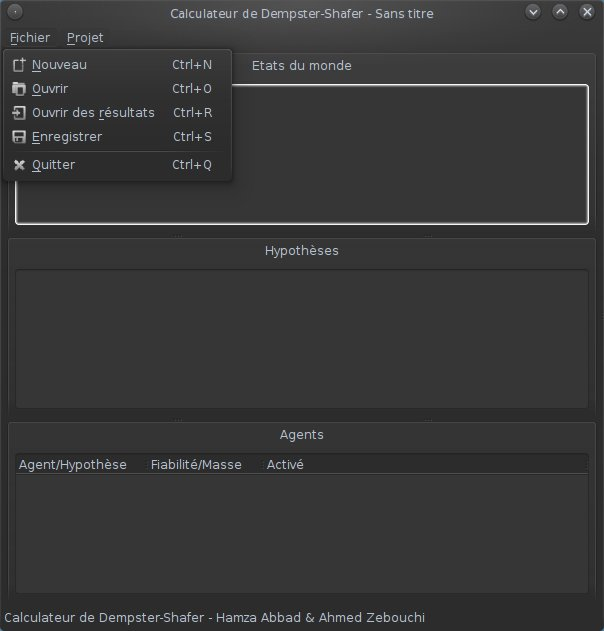
\includegraphics[width=\textwidth]{Inetrface_principale_menu_fichier}
\caption{Le menu \textbf{Fichier}}
\end{subfigure}
\hfill
\begin{subfigure}{0.49\textwidth}
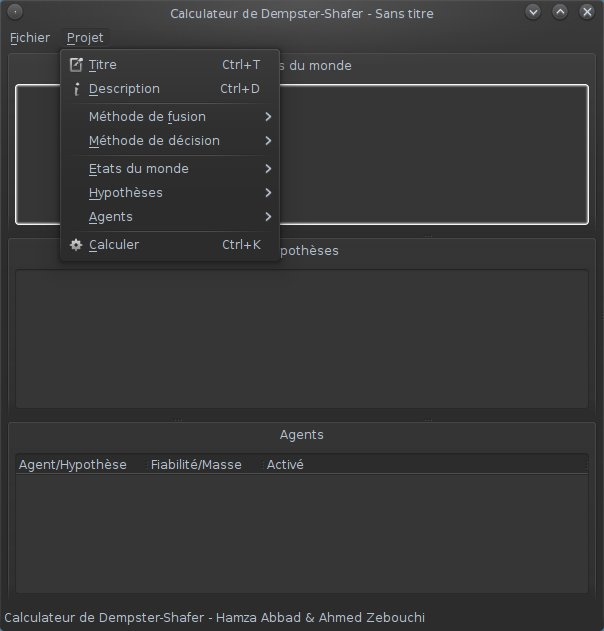
\includegraphics[width=\textwidth]{Inetrface_principale_menu_projet}
\caption{Le menu \textbf{Projet}}
\end{subfigure}
\caption{L'interface principale du \appname}
\end{figure}

Les états du monde, les hypothèses et les agents doivent s'ajouter dans cet ordre à partir
de ce menu ou par un clic droit dans leurs champs. \`A partir de ce menu, l'utilisateur a la possibilité de sélectionner une
des méthodes de fusion: \textit{Dempster-Shafer}, \textit{Dubois-Prade}, \textit{Smets} ou
\textit{Yager}. Il peut aussi choisir la méthode de décision qui sera utilisée parmi les trois
suivantes: \textit{Optimiste}, \textit{Pessimiste} ou \textit{Pignistique}.

La première étape consiste à ajouter tous les états du monde. Ensuite, chaque fois qu'un ensemble d'états est sélectionné
l'hypothèse correspondante est établie.\\[1em]

\begin{figure}[H]
\begin{subfigure}{0.49\textwidth}
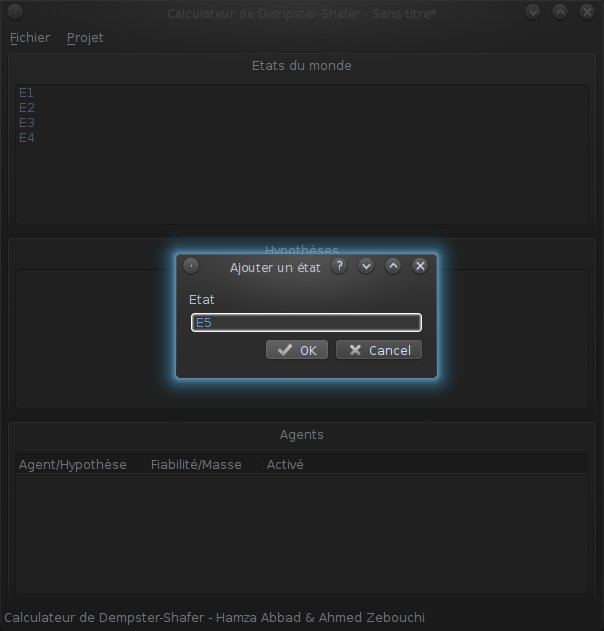
\includegraphics[width=\textwidth]{ajouter_etat}
\caption{Ajouter les états du monde}
\end{subfigure}
\hfill
\begin{subfigure}{0.49\textwidth}
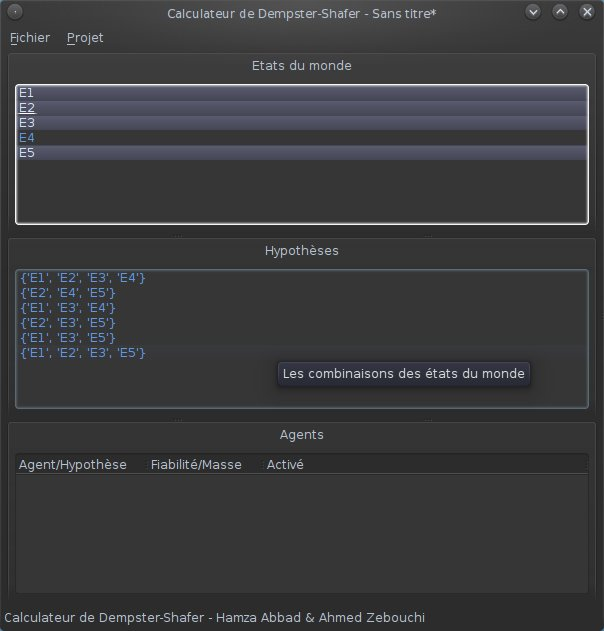
\includegraphics[width=\textwidth]{ajouter_hypothese}
\caption{Ajouter une hypothèse à partir des états}
\end{subfigure}
\caption{L'ajout des états du monde et les hypothèses}
\end{figure}

Par la suite, l'utilisateur doit procéder à l'ajout des agents. Chaque agent doit avoir un nom, un niveau de
fiabilité et un ensemble d'hypothèses tel que à chaque hypothèse est affectée une masse entre
$0$ et $1$.\\[1em]

\begin{figure}[H]
\begin{subfigure}{0.49\textwidth}
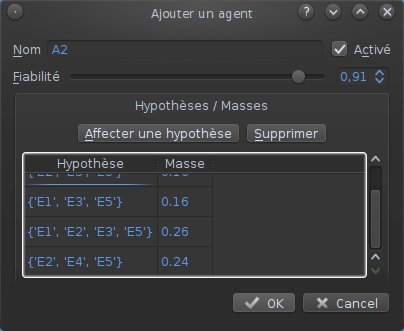
\includegraphics[width=\textwidth]{ajouter_agent}
\caption{Dialogue de l'ajout d'un agent}
\end{subfigure}
\hfill
\begin{subfigure}{0.49\textwidth}
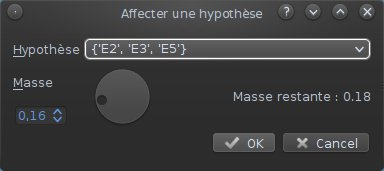
\includegraphics[width=\textwidth]{affecter_masse}
\caption{Dialogue de l'affectation d'une hypothèse}
\end{subfigure}
\caption{L'ajout d'un agent et l'affectation de ses hypothèses}
\end{figure}

Avant de passer au calcul, les données saisies doivent être enregistrées dans un fichier à l'aide de la fonctionnalité
\textbf{Enregistrer} ou \textbf{Enregistrer sous}. Il faut aussi choisir un nom et un emplacement pour le
fichier. Il aura par défaut l'extention \texttt{.dsti.xml}. Cette action est nécessaire car elle génère
le fichier d'entrée pour le noyau. Si cette étape est ignorée, le programme demandera de la faire avant de
continuer.\\[1em]

\begin{figure}[H]
\centering
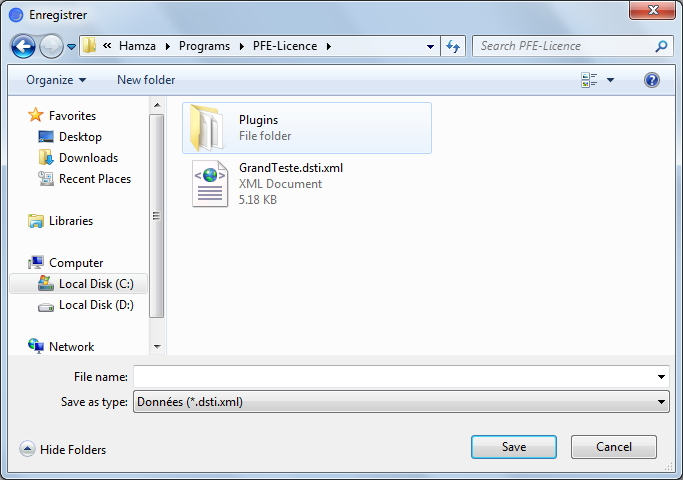
\includegraphics[width=0.8\textwidth]{Enregistrer}
\caption{Enregistrer les données}
\end{figure}

La dernière étape consiste à lancer le calcul. Cette étape risque de prendre un temps important si le nombre des états
du monde et/ou des agents est assez grand. Pour cela, un dialogue d'attente est affiché pendant l'exécution
du noyau en arrière-plan. L'utilisateur peut annuler cette opération à tout moment en cliquant sur le bouton
\emph{Annuler}.

Quand le calcul se termine, un dialogue contenant les informations du projet et tous les résultats sera affiché.
Les résultats sont obtenus par la lecture du fichier généré par le noyau qui a le même chemin que le fichier
sauvegardé, sauf qu'il porte l'extention \texttt{.dsto.xml}. Ce dialogue permet de rechercher une hypothèse en
tapant une partie de son nom dans la zone de texte qui contient le mot \emph{Rechercher}.
Les hypothèses qui correspondent à l'entrée de l'utilisateur sont sélectionnées afin de faciliter
la recherche. Il y a aussi un bouton permettant de créer un nouvel agent et de remplir ses hypothèses et ses masses
à partir de celles affichées. L'utilisateur doit introduire le nom de cet agent.

\begin{figure}[H]
\begin{subfigure}{0.39\textwidth}
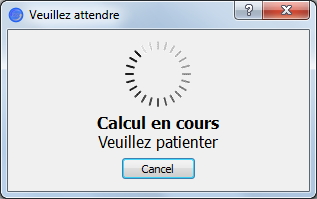
\includegraphics[width=\textwidth]{Dialogue_attente}
\caption{Dialogue d'attente}
\end{subfigure}
\hfill
\begin{subfigure}{0.59\textwidth}
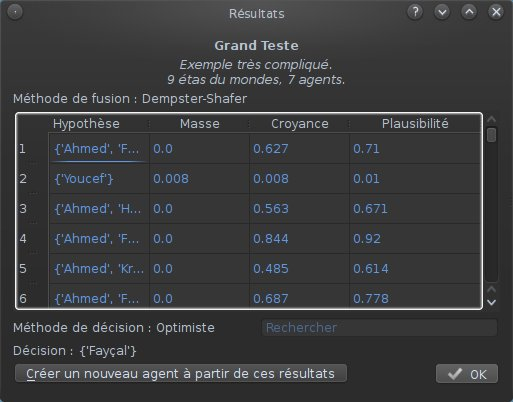
\includegraphics[width=\textwidth]{Dialogue_resultats}
\caption{Dialogue des résultats}
\end{subfigure}
\caption{Le calcul et l'affichage des résultats}
\end{figure}

Par la suite, les fichiers de données peuvent être accessibles en utilisant l'action \textbf{Ouvrir} à partir
du menu fichier. Les résultats peuvent être aussi affichés en ouvrant le fichier correspondant en utilisant l'action
\textbf{Ouvrir des résultats}.

\begin{figure}[H]
\begin{subfigure}{0.49\textwidth}
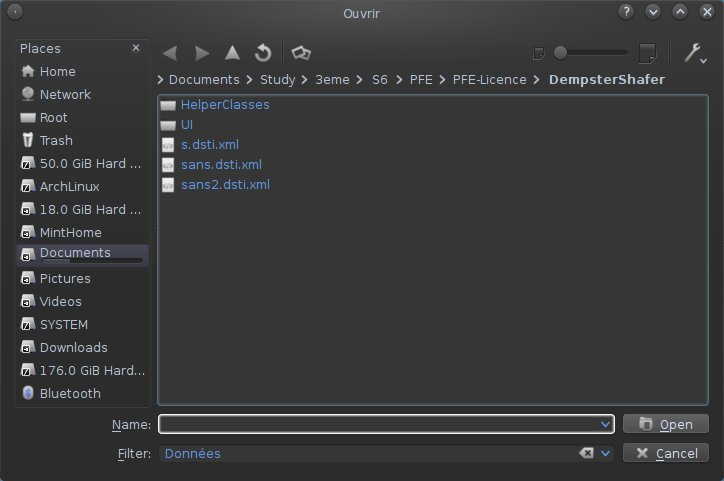
\includegraphics[width=\textwidth]{Ouvrir}
\caption{Dialogue d'ouverture d'un fichier de données}
\end{subfigure}
\hfill
\begin{subfigure}{0.49\textwidth}
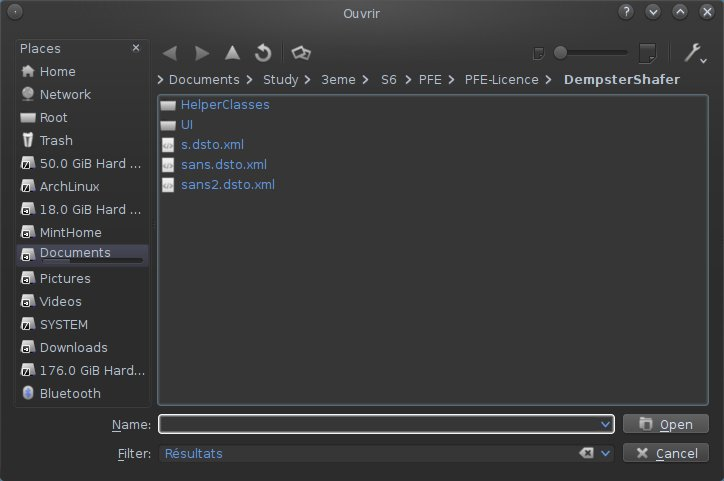
\includegraphics[width=\textwidth]{Ouvrir_resultats}
\caption{Dialogue d'ouverture de résultats}
\end{subfigure}
\caption{Les dialogues de l'ouverture d'un fichier}
\end{figure}

\section{La \platformename}

Ce programme est une interface composée de plusieurs panneaux et chaque panneau est accessible
à partir de son titre dans la barre des onglets. Un panneau comporte une ou plusieurs interfaces pour
un ou plus d'un programme externe.  La \platformename est facilement extensible; pour ajouter un nouveau
panneau dans cette interface il suffit de créer une classe personnalisée qui dérive de la classe
\mbox{\texttt{javax.swing.JPanel}} dans le paquet \texttt{Plugins}. Jusqu'à présent, la \platformename
contient quatre onglets : \textit{Imprécision}, \textit{Décision}, \textit{Incertain}
et \textit{Tools}.

Dans le panneau \textit{Imprécision} il y a un bouton pour lancer la \textbf{Fuzzy Logic Toolbox} qui est une
bibliothèque de \textit{MATLAB} avec une interface graphique intégrée facilitant l'exploitation directe
de la bibliothèque.

\begin{figure}[H]
\centering
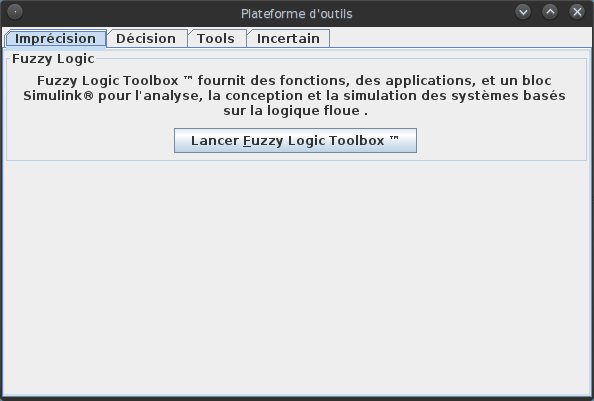
\includegraphics[width=0.7\textwidth]{Imprecision}
\caption{Le panneau \textbf{Imprécision}}
\end{figure}

Le panneau \textit{Décision} contient deux parties, l'une appelée \textit{Logique}
contenant un bouton pour exécuter l'application \textbf{DecPos} qui permet de calculer la décision optimale dans
le cas pessimiste ou optimiste et d'effectuer autres opérations sur les bases possibilistes; l'autre qui
s'appelle \textit{Graphique} qui contient un bouton pour exécuter l'application \textbf{GraphViz02} pour
le traitement des graphes de décision.

\begin{figure}[H]
\begin{subfigure}{0.49\textwidth}
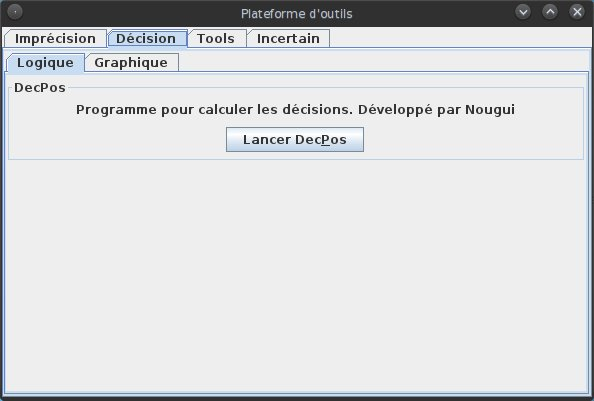
\includegraphics[width=\textwidth]{Decision_logique}
\caption{La partie \textbf{Logique}}
\end{subfigure}
\hfill
\begin{subfigure}{0.49\textwidth}
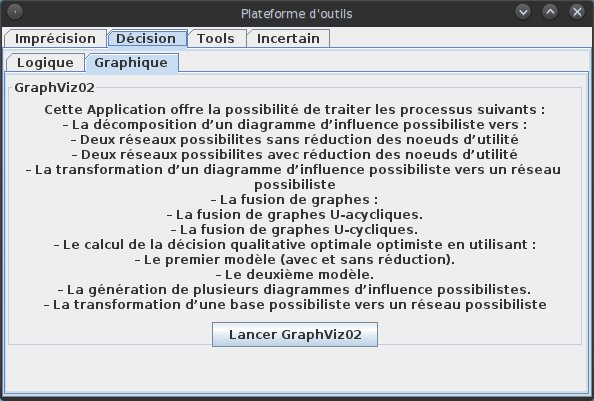
\includegraphics[width=\textwidth]{Decision_graphique}
\caption{La partie \textbf{Graphique}}
\end{subfigure}
\caption{Le panneau \textbf{Décision}}
\end{figure}

\vspace*{1.5em}
Le panneau \textit{Incertain} regroupe les interfaces nécessaires pour dessiner un graphe orienté sans
cycles de nature BNT ou PNT et pour modifier ses paramètres après la validation. Il y a un bouton \textbf{Ajouter un noeud}
permettant d'ajouter un nouveau nœud isolé. Les noeuds doivent être reliés par des arcs qui sont créés par le
glissement du curseur à partir d'un noeud et le relâchement dans un autre. Ensuite, l'utilisateur doit valider le graphe
en utilisant le bouton \textbf{Valider} et puis il doit changer les paramètres de chaque noeud et spécifier la vraissemblance,
le noeud observé, et ajouter les évidences. Enfin il peut générer un script \textit{MATLAB} et de l'exécuter en cliquant
sur le bouton \textbf{Calculer}.
\vspace*{3em}

\begin{figure}[H]
\centering
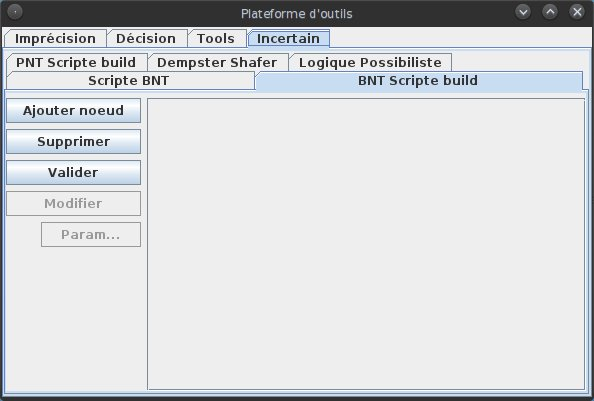
\includegraphics[width=0.7\textwidth]{Incertain_BNT_graphe}
\caption{L'interface du graphe BNT}
\end{figure}
\vspace*{2em}

Dans le même panneau, il y a aussi un panneau interne qui porte le nom \textit{Dempster-Shafer} pour exécuter
notre application \appname qui a été présentée auparavant. Le dernier panneau est celui de \textit{Logique possibiliste}.
Il représente une interface pour un ensemble des programmes qui seront exécutés en série. Il permet de spécifier le nombre
de noeuds dans un graphe possibiliste et le nombre maximal de parents pour chaque noeud, ainsi que le nombre de propositions
(1 ou 2). Le programme génère un graphe aléatoire par lancement d'un script \textit{MATLAB} suivi par deux programmes
\texttt{passage} et \texttt{inference}. Enfin, il affiche les résultats pour l'utilisateur.

\begin{figure}[H]
\begin{subfigure}{0.49\textwidth}
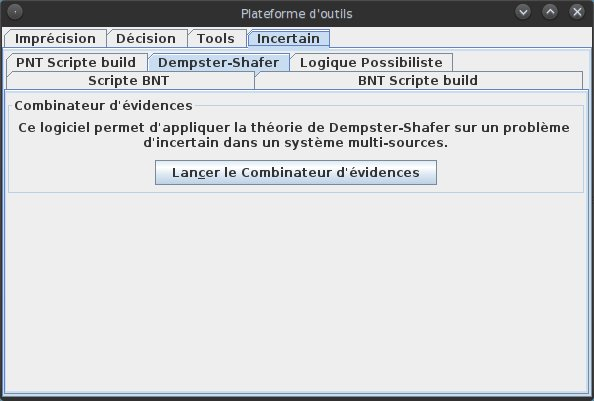
\includegraphics[width=\textwidth]{Incertain_DS}
\caption{Le panneau interne \textbf{Dempster-Shafer}}
\end{subfigure}
\begin{subfigure}{0.49\textwidth}
\hfill
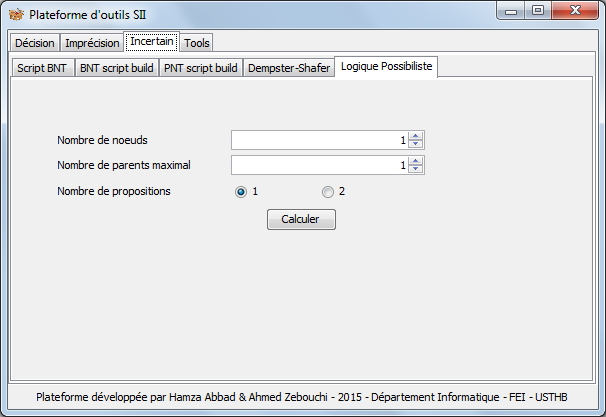
\includegraphics[width=\textwidth]{Incertain_LP}
\caption{Le panneau interne \textbf{Logique possibiliste}}
\end{subfigure}
\caption{Le panneau \textbf{Incertain}}
\end{figure}

Le dernier panneau \textit{Tools} contient deux interfaces pour utiliser le logiciel \textbf{UBCSAT}, la
première pour calculer le SAT et la deuxième pour le Weighted Max SAT. L'utilisateur doit introduire les formules
logiques sous forme FND\footnote{Forme normale disjonctive}.

\begin{figure}[H]
\centering
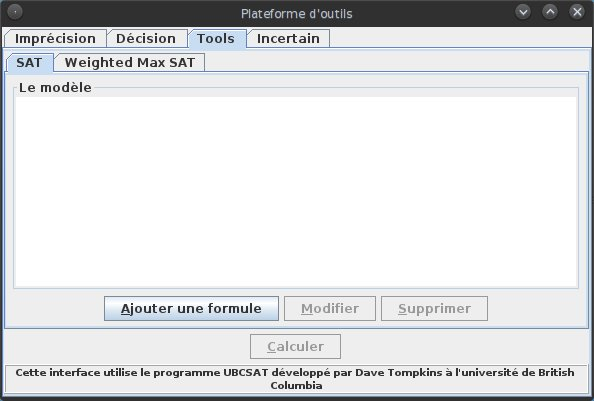
\includegraphics[width=0.7\textwidth]{Tools_SAT}
\caption{Le panneau \textbf{Tools}}

\end{figure}
\vspace*{-2em}
\phantomsection
\addcontentsline{toc}{section}{Conclusion}
\section*{Conclusion}

Nous avons présenté globalement ce que nous avons réalisé dans notre projet. Nous avons commencé par une
présentation détaillée de notre application \appname que nous avons entièrement développée, et puis, nous
avons montré les différentes tâches qui peuvent être réalisées à travers notre interface \platformename.

\end{document}          
